In this chapter we describe how we predict the position of periods, commas and question marks in unpunctuated text using lexical features.
The used data is described in Section \ref{sec:training_data}.

The system is based on the deep learning framework \emph{caffe}.
Therefore the processing pipeline is the following:

\begin{itemize}
\item preprocess the data, so that it can be used as input for caffe
\item train the network with the preprocessed data
\item retrieve predictions for new data
\item transform the output into a valuable result
\end{itemize}

\subsection{Data Preprocessing}

For processing the data, we need to extract features which caffe can handle.
Since you can not use a whole text as input, we decided to use a sliding window to generate training and testing instances.
A sliding window is in our case, that we split a sentence like \emph{The sun is shining and we go outside} into the following pieces (assuming a window size of 5):
\begin{itemize}
\item the sun is shining and
\item sun is shining and we
\item is shining and we go
\item shining and we go outside
\end{itemize}

We call these pieces instances and the window size directly defines how many words are in each instance.
The label of each instance is then whether there is a punctuation (and which one) at a defined position.
We call this position punctuation position.
In the above example every instance would have a label of \emph{None} with a punctuation position of 2, since there is no punctuation.

After we split up the sentences into instances we convert each word into a distributed word representation.
We use the distributed word representation described earlier: \emph{word2vec}. \todo{Insert word2vec link. Describe Word2Vec in related work?}
The final model we used for our distributed word representation was trained on google news entries \todo{Link and/or paper}.
Since not every word exists in the trained model, we use the word vector representing \emph{this} for unknown words.
We think that most of the unknown words are proper names, which can easily be replaced with \emph{this} without changing the meaning and structure of the whole sentence.

We also figured out that the trained model only contains the number \emph{1} and a few more of the most common numbers instead of all numbers. \todo{Check whether only 1 is in the word vector or whether numbers like 12 and 5 are also contained}
That is why we replace any number with \emph{1}.

The representation for each word in an instance is inserted into one row of the feature matrix, e.g. for a sliding window size of 5 you get the matrix of 5x300 for each instance.

Besides the distributed word representation we also examined Part of Speech (POS) tags as features.
We used the nltk POS tagger to identify the POS tags with the whole text as input.
The tagger distinguishes between 35 different POS tags.
These are too specific for our purpose, so we reduced them into 14 different categories.
For example we combined CD and LS to a more generic category \emph{numeral}.
The nltk tagger predicts more than one tag per word, so one word can have multiple tags (even after reducing the tag categories).
To allow the existence of multiple tags in our feature matrix, we used the following representation:
We create one flag per POS category which has the value 1 if the word belongs to this category and 0 otherwise.

There are two possibilities to include them.
On the one hand it is possible to append all flags at the end to word vector representations.
On the other hand an extra channel with the flags can be used.

For all further testing, wherever we used the POS-features, we decided to append the flags to the vector representation of the words.
Therefore the resulting feature matrix for a sliding window size of 5 with POS tags is 5x314.

% Data preparation
% Windowing
% Config.ini File

% Google Vector

\subsection{Neural Network Layout}
Describe the net, the features

\subsection{Evaluation}
Formeln für Precision, Recall, Harmonic Mean
Evaluation, wikipidia usage?, results with wikipedia test set

Evaluation of results:
\begin{itemize}
\item F-measure for each class is calculated.
\item Harmonic mean for all F-measures is total score (higher is better).
\end{itemize}

\begin{figure}[ht]
    \centering
    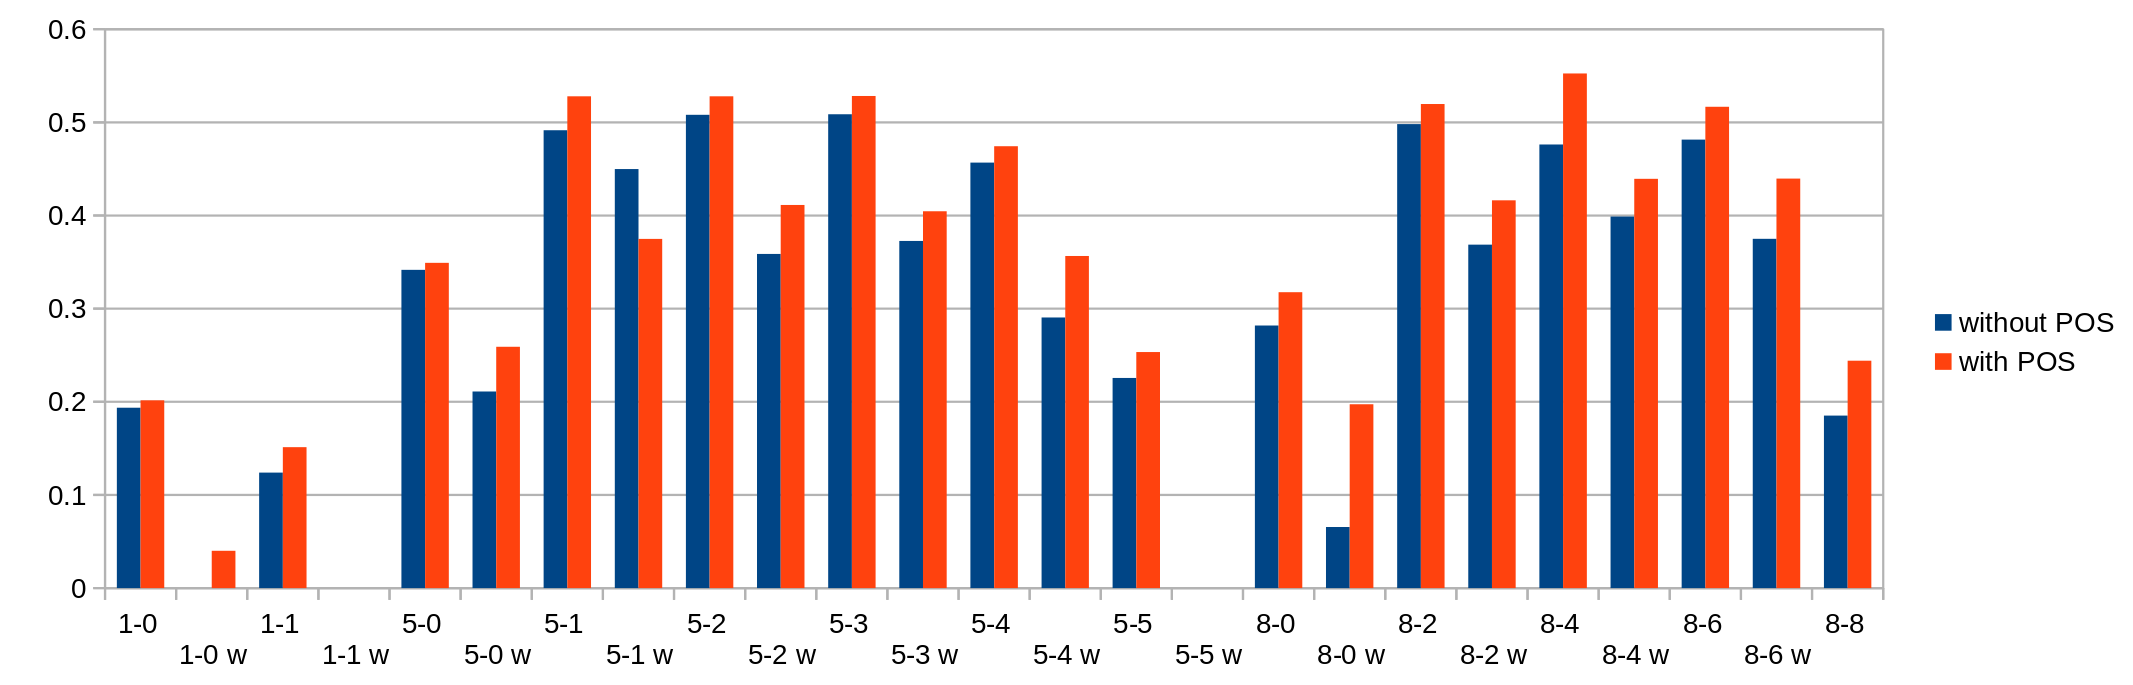
\includegraphics[width=\textwidth]{img/window_eval.png}
    \caption{Harmonic mean between all f1 scores for all classes. \emph{2/5} means window size of five and punctuation is tested at position two. If \emph{wi} is in the label, it uses wikipedia training data.}
    \label{window_eval}
\end{figure}

\begin{figure}[ht]
    \centering
    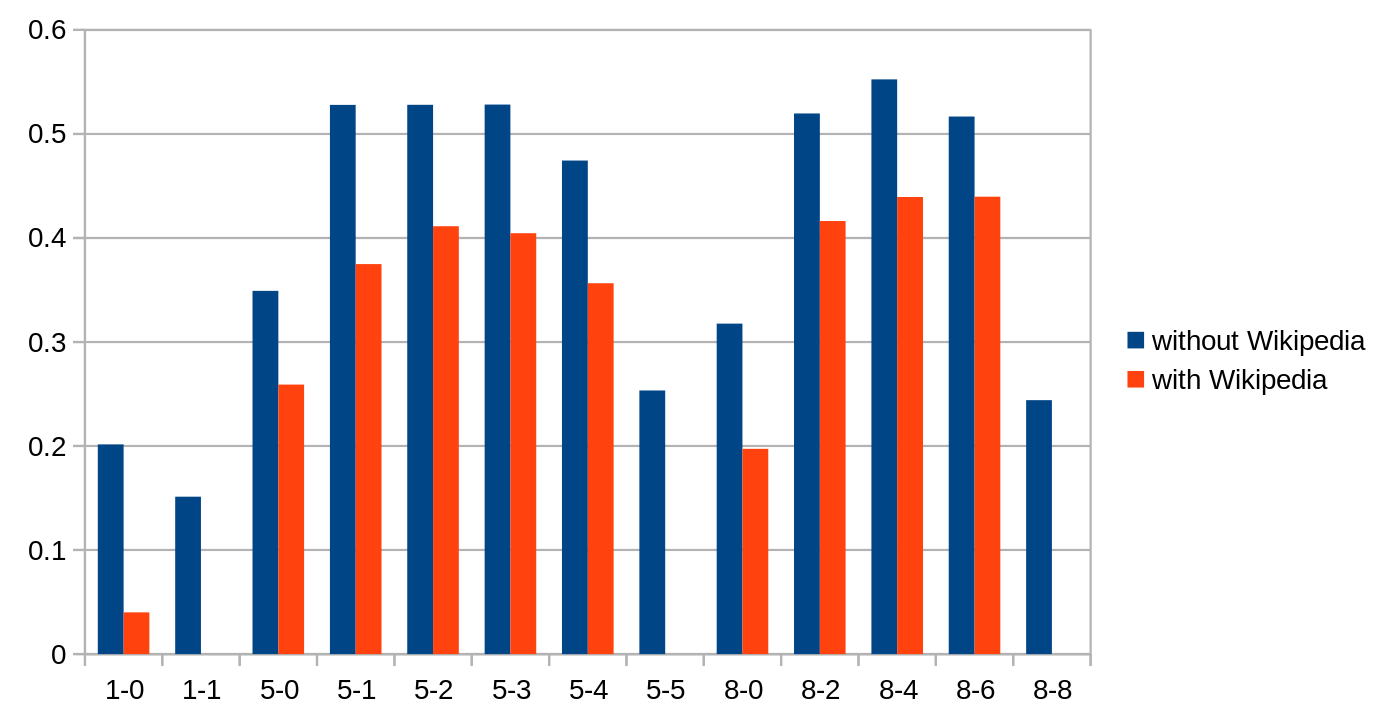
\includegraphics[width=\textwidth]{img/window_wiki_eval.png}
    \caption{}
    \label{window_wiki_eval}
\end{figure}

\begin{figure}[ht]
    \centering
    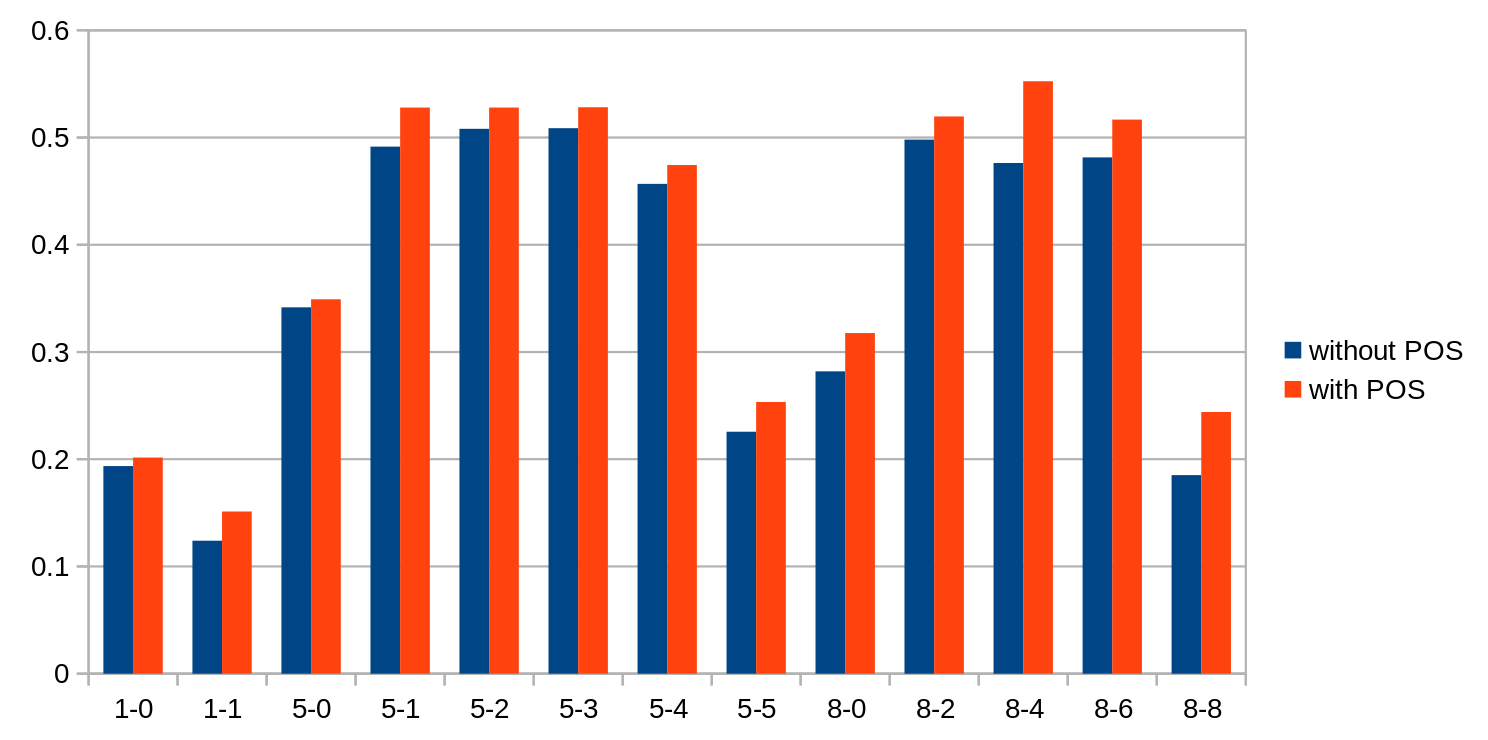
\includegraphics[width=\textwidth]{img/window_pos_eval.png}
    \caption{}
    \label{window_pos_eval}
\end{figure}

Comparison between experiments with and without POS tagging (other than that, they have the same configurations):
\begin{itemize}
\item With POS tagging: 0.305
\item Without POS tagging: 0.275
\end{itemize}

Comparison between experiments with and without wikipedia data (other than that, they have the same configurations):
\begin{itemize}
\item Without wikipedia: 0.385
\item With wikipedia data: 0.252
\end{itemize}
